\begin{figure*}[!p]
\centering
\begin{minipage}[b]{.42\textwidth}
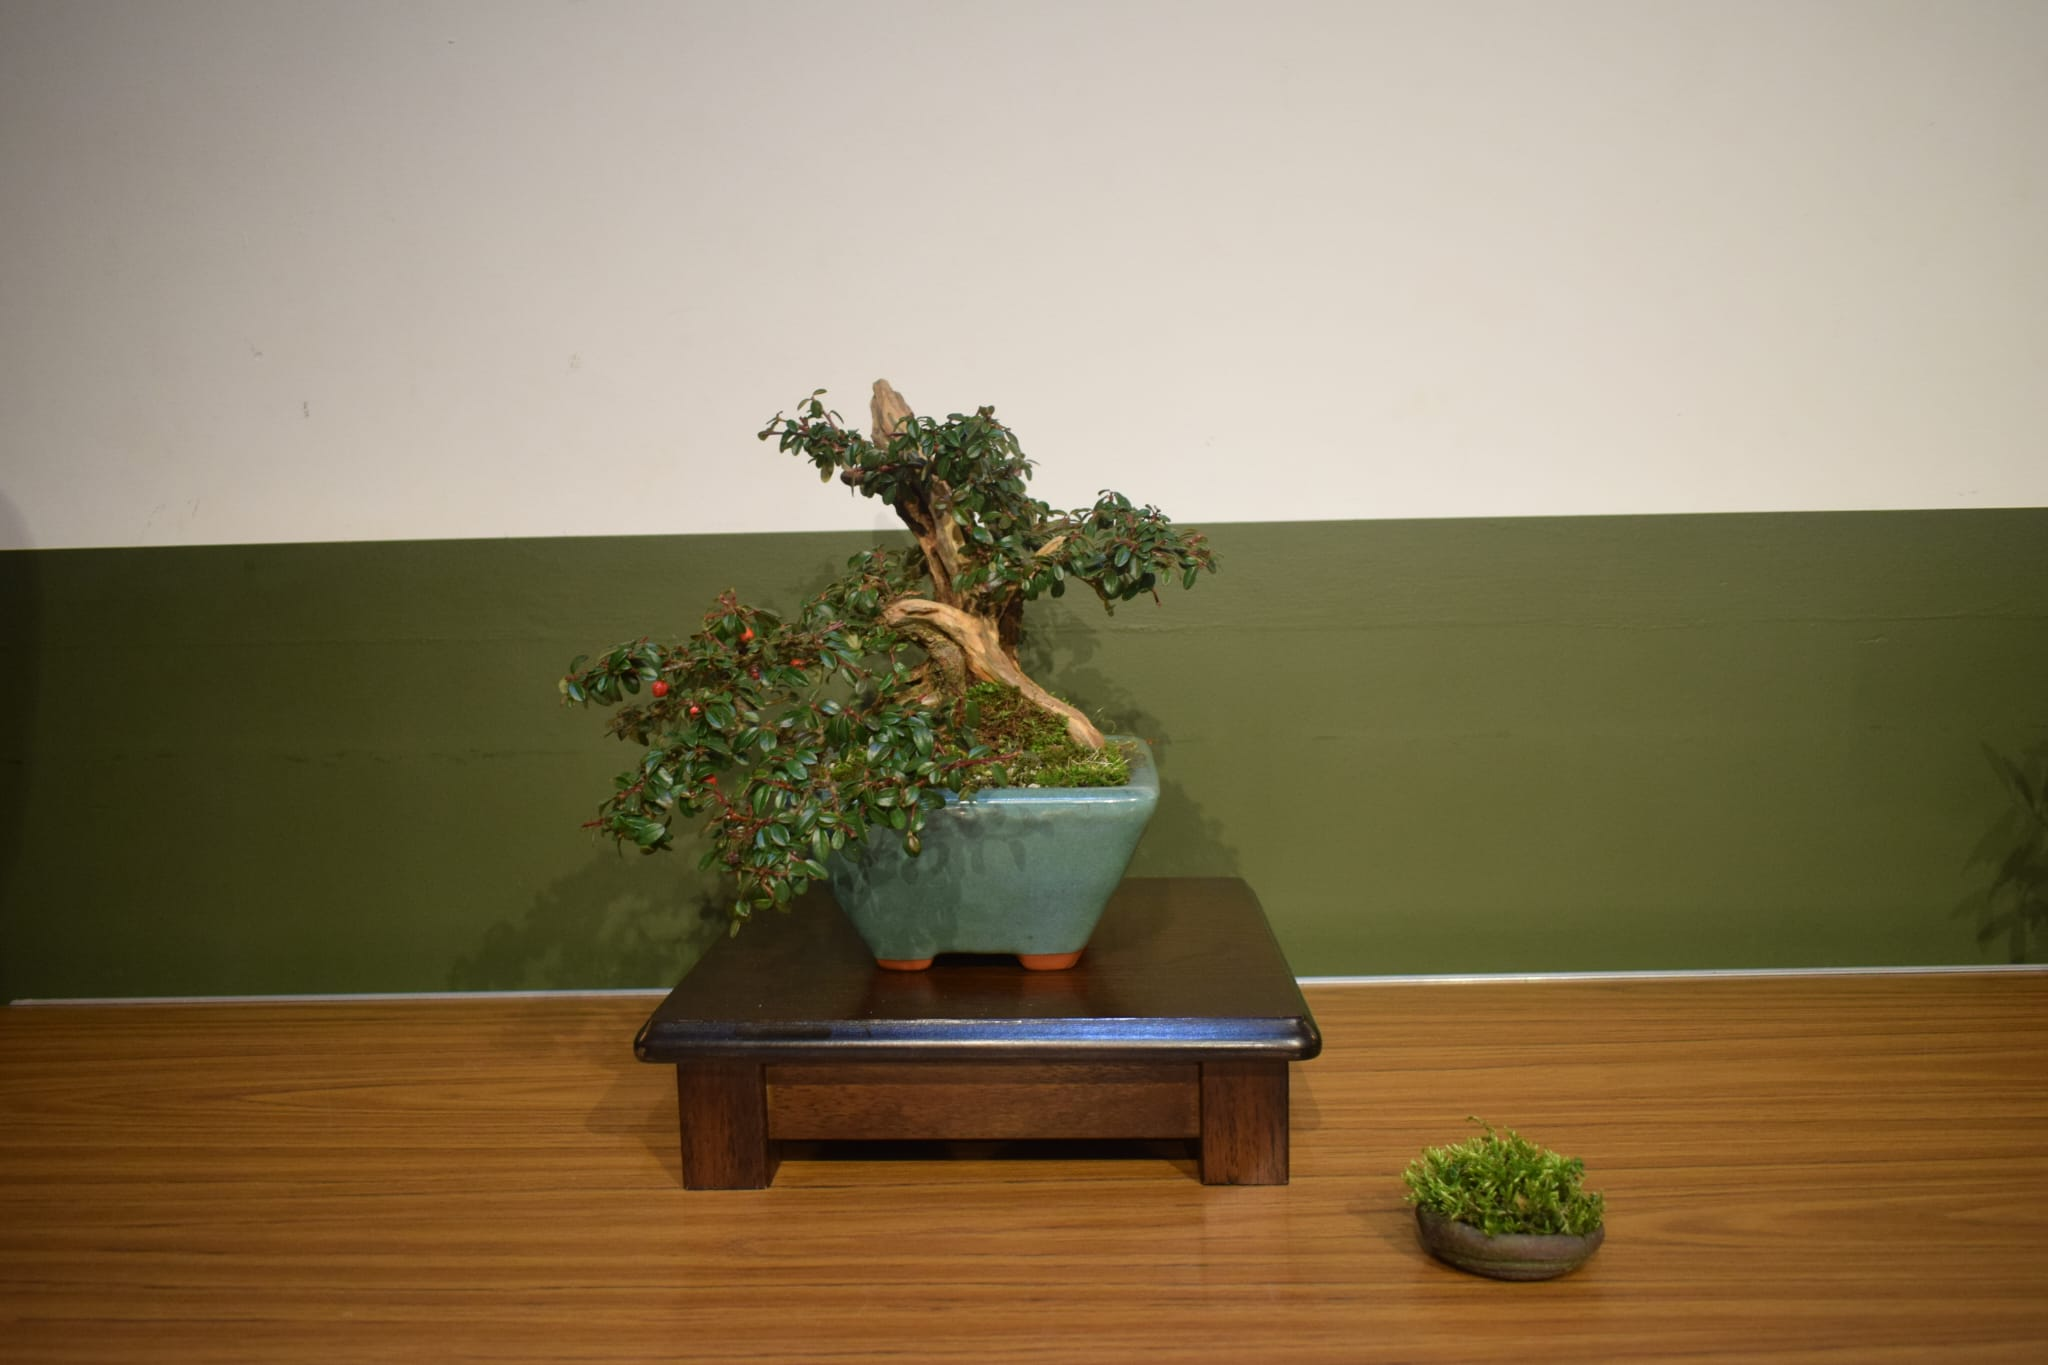
\includegraphics[width=1.0\textwidth]{2025_02/res/contest_david_cotoneaster}
\centerline{\emph{David's Cotoneaster.}}
\end{minipage}\qquad
\begin{minipage}[b]{.42\textwidth}
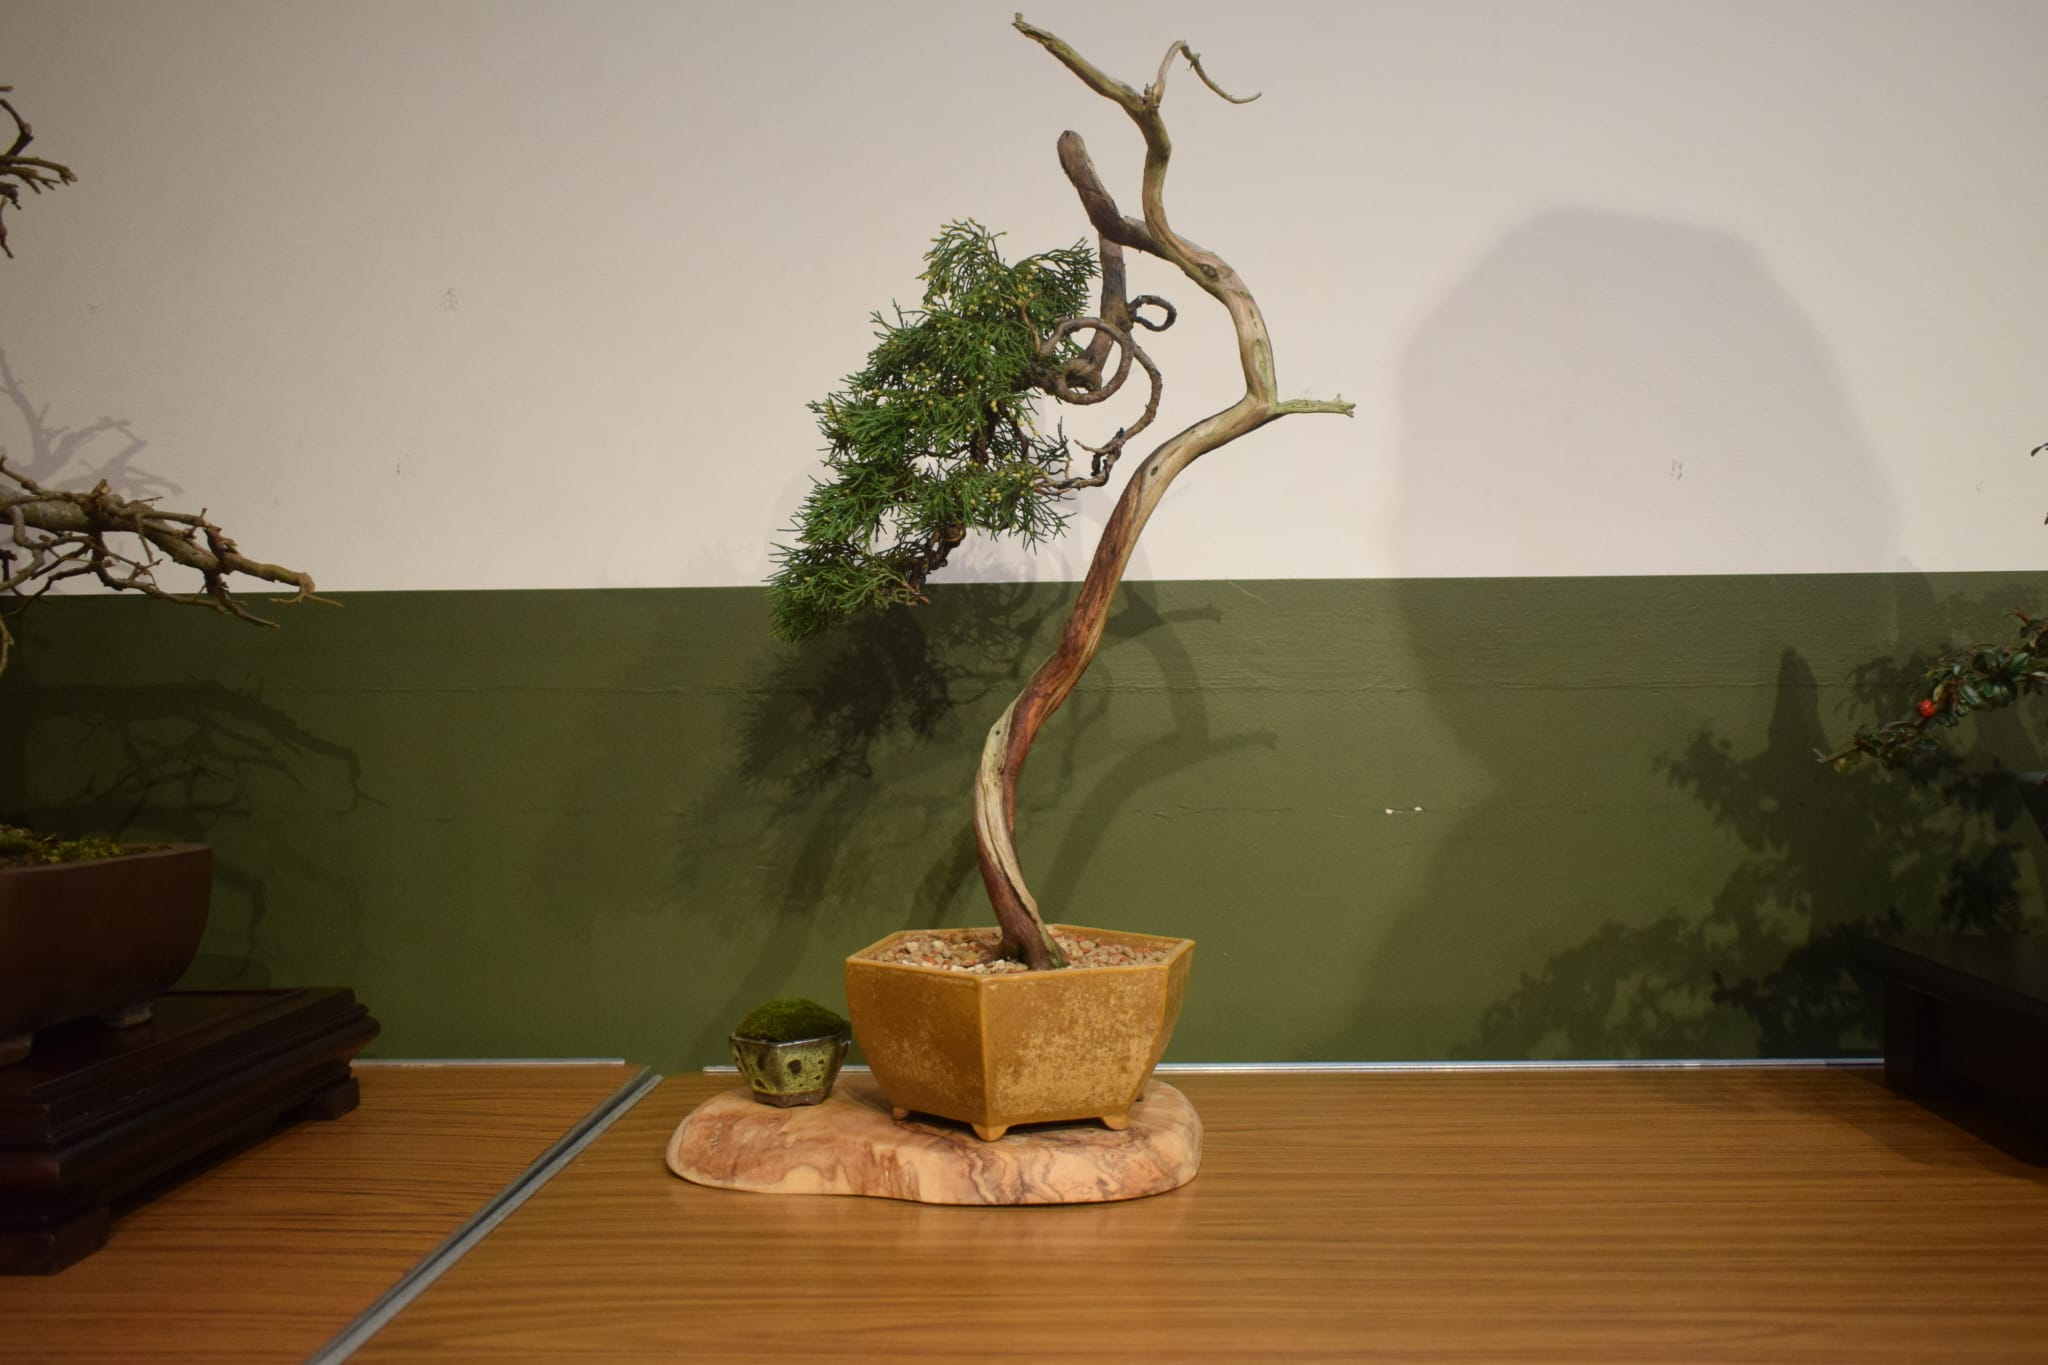
\includegraphics[width=1.0\textwidth]{2025_02/res/contest_brendan_juniper}
\centerline{\emph{Brendan's Juniper Sabina.}}
\end{minipage}

\begin{minipage}[b]{.42\textwidth}
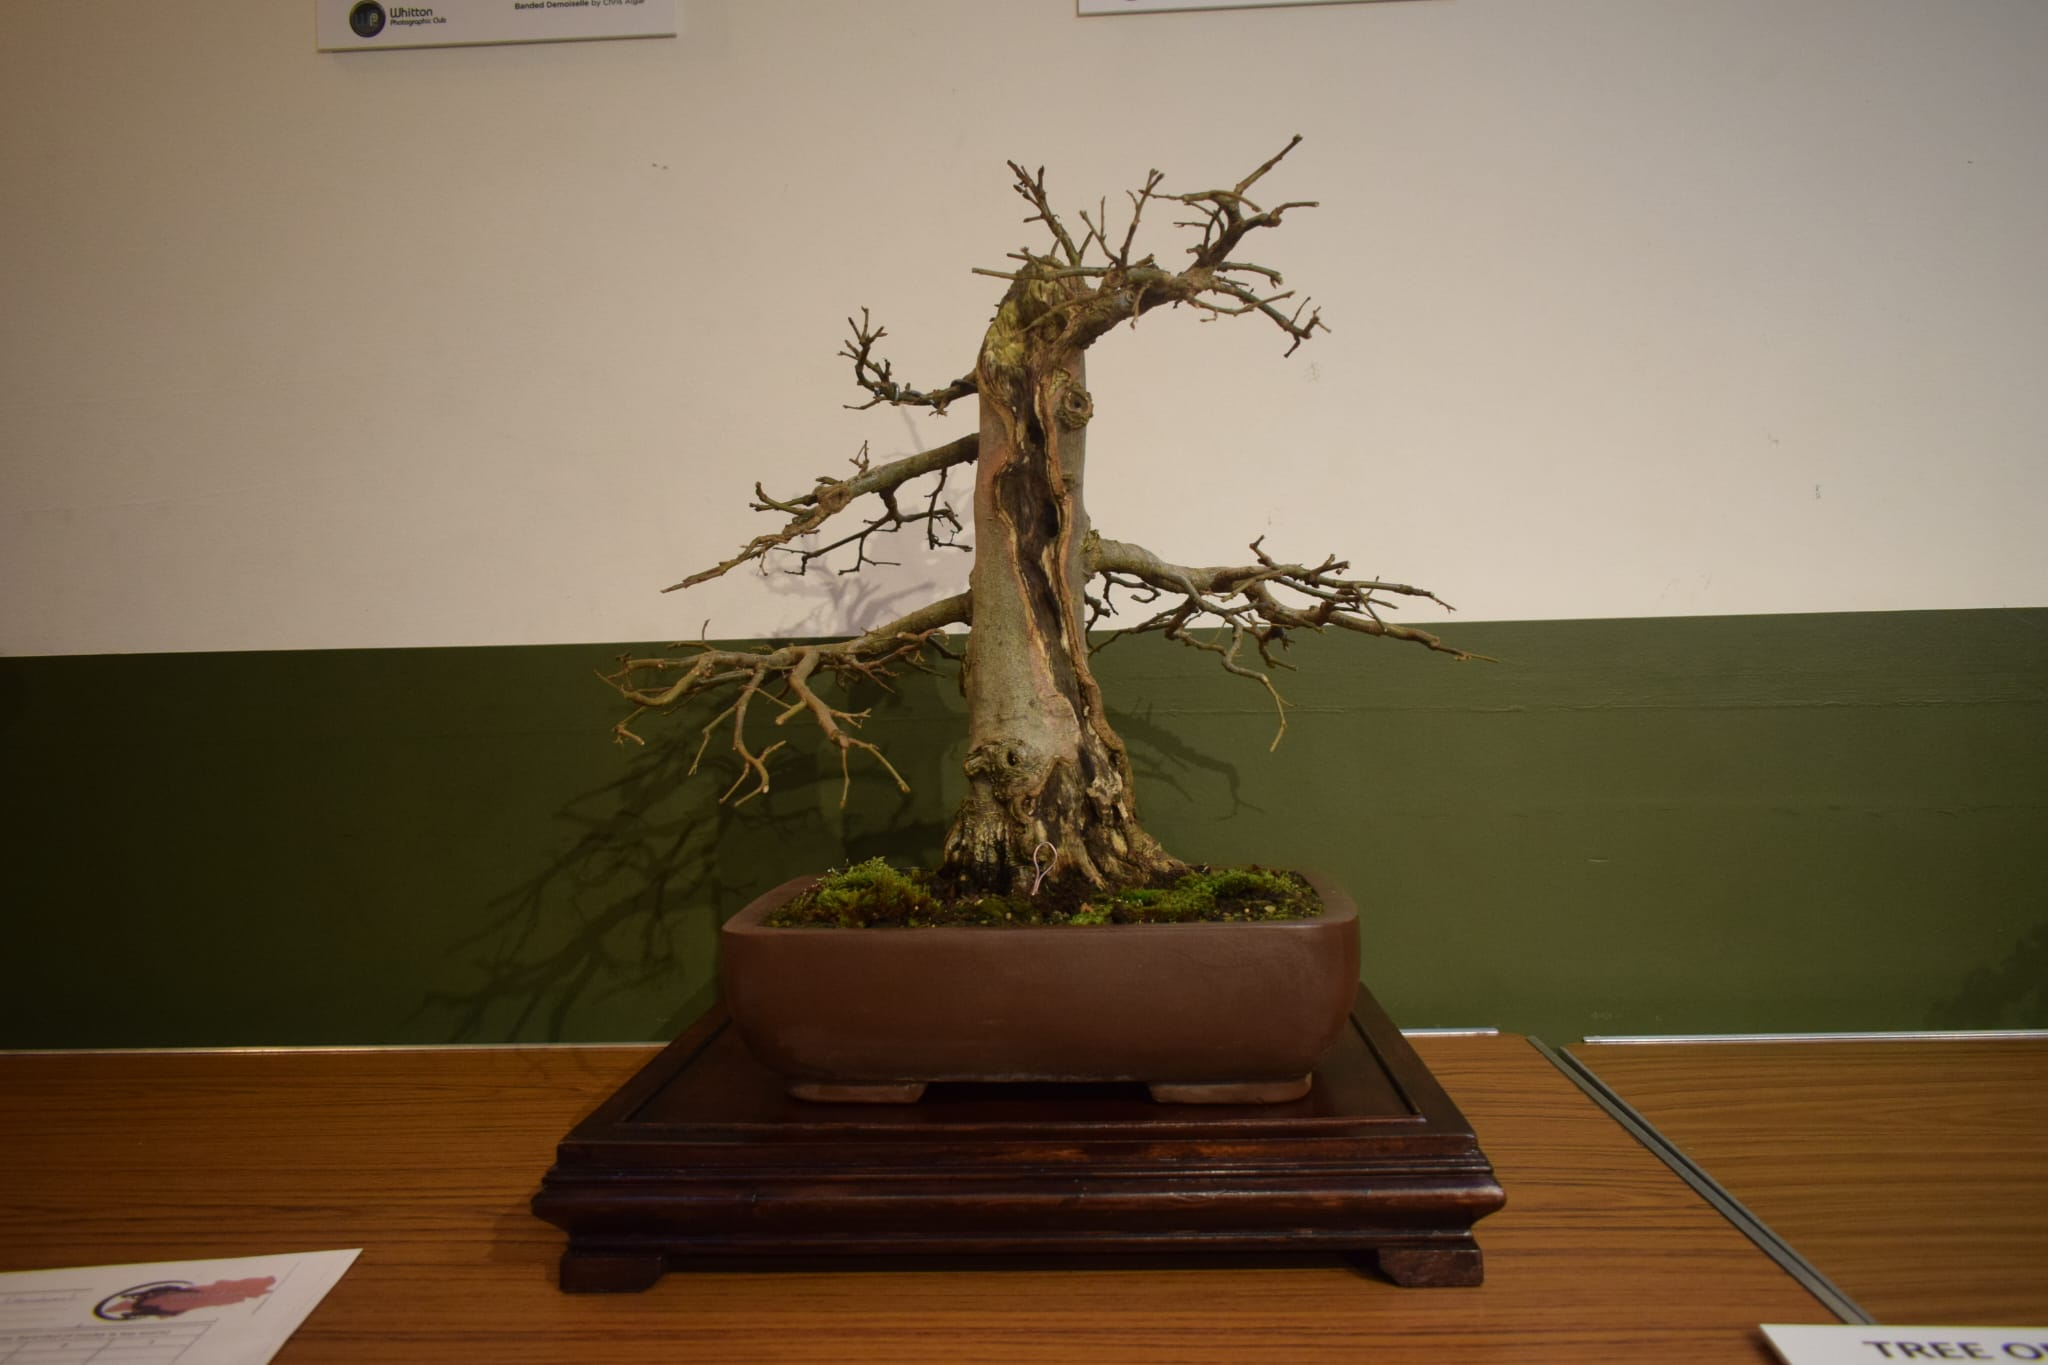
\includegraphics[width=1.0\textwidth]{2025_02/res/contest_terry_hornbeam}
\centerline{\emph{Terry's Hornbeam.}}
\end{minipage}\qquad
\begin{minipage}[b]{.42\textwidth}
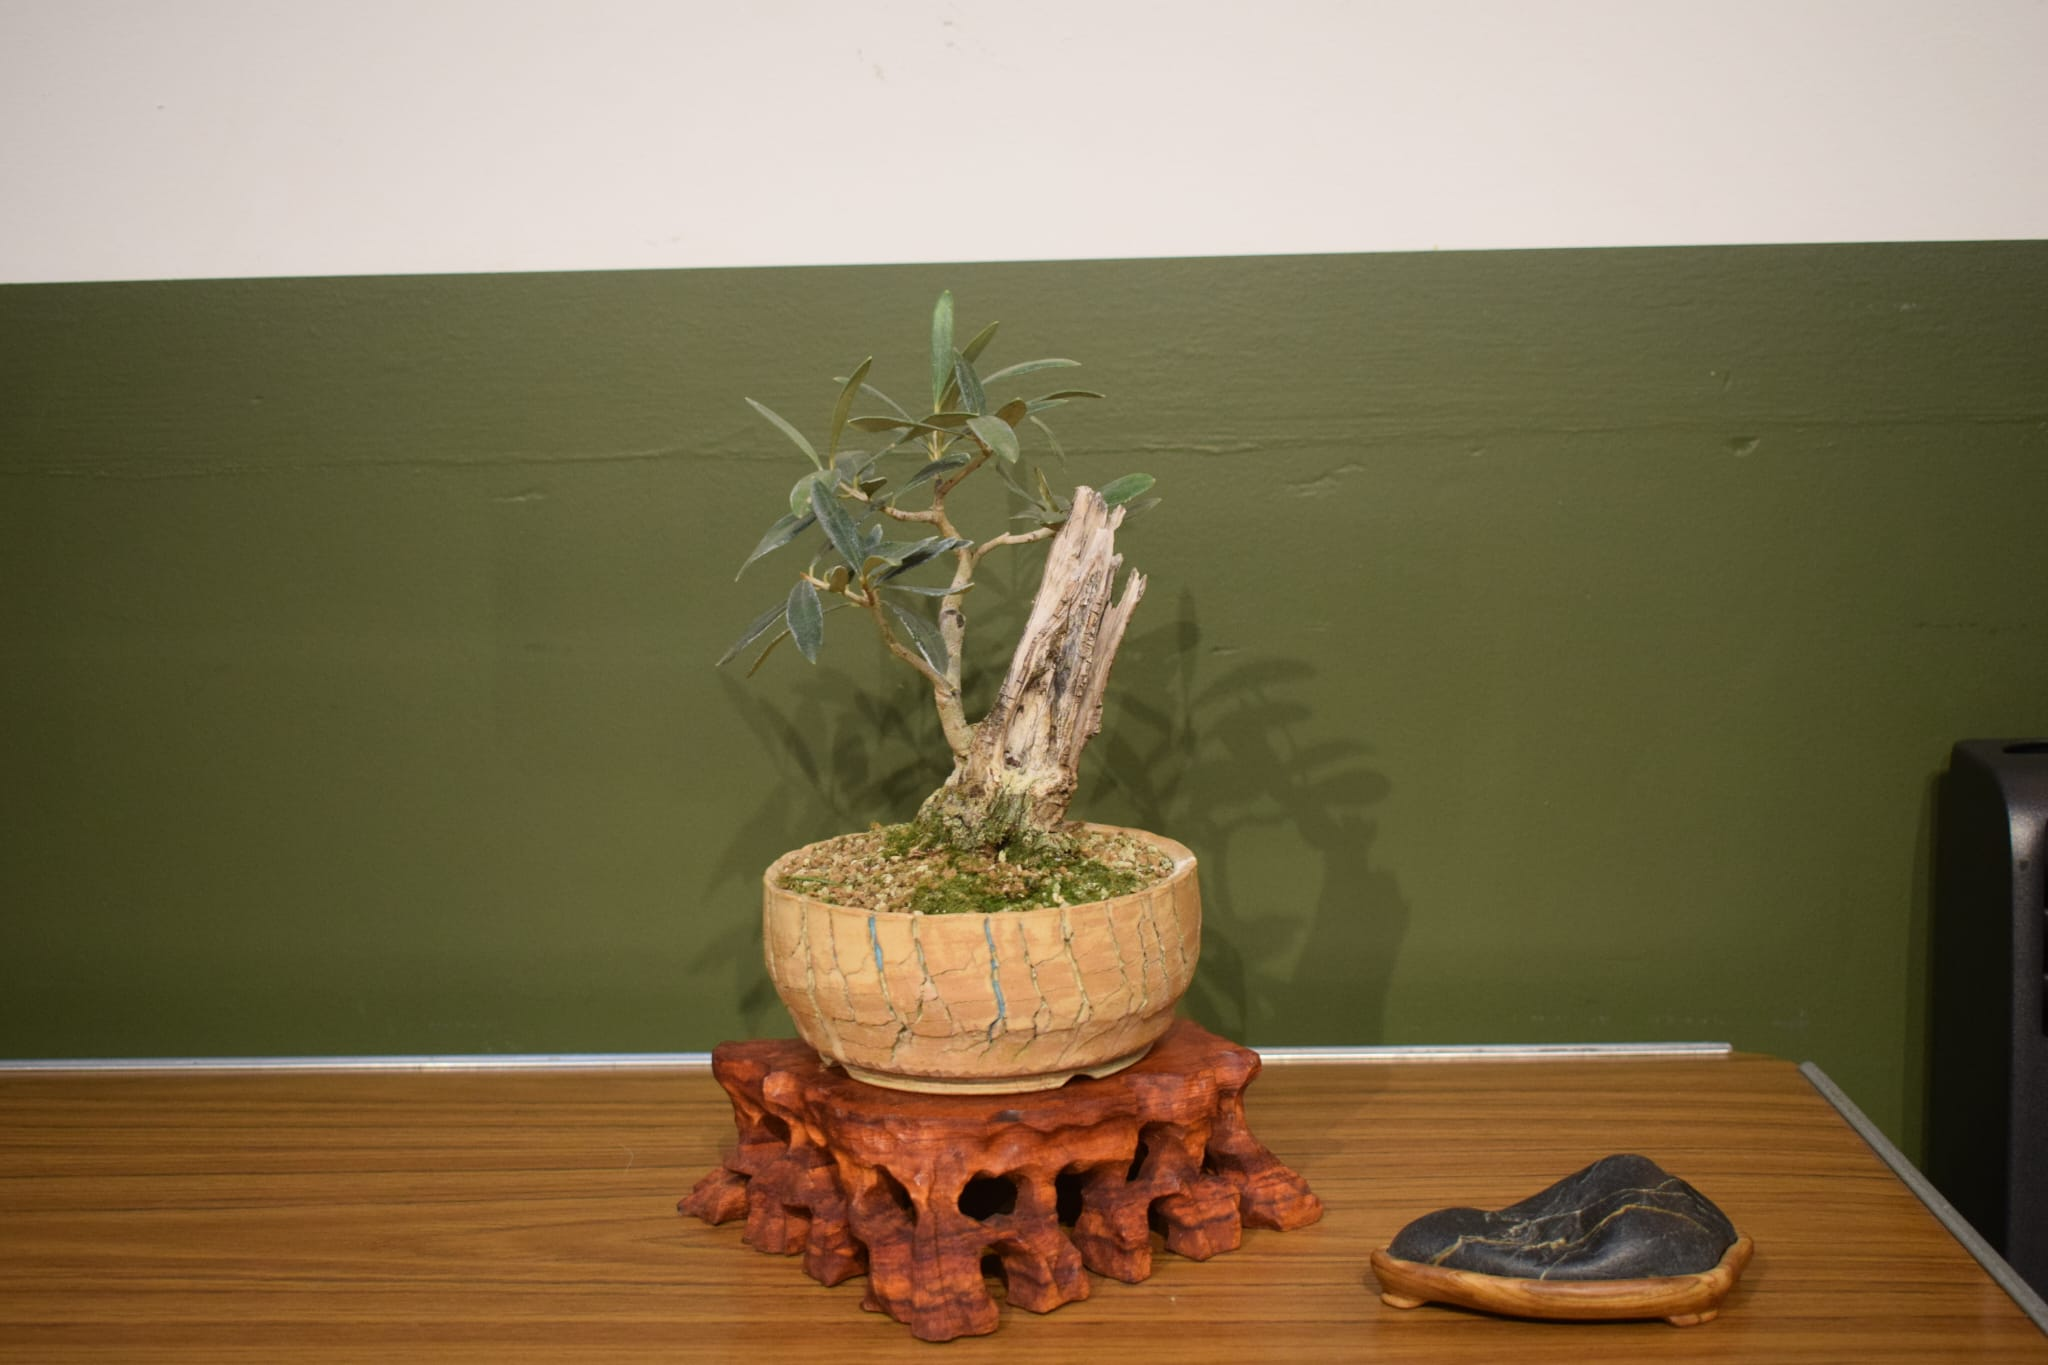
\includegraphics[width=1.0\textwidth]{2025_02/res/contest_rory_olive}
\centerline{\emph{Rory's Olive tree.}}
\end{minipage}

\begin{minipage}[b]{.42\textwidth}
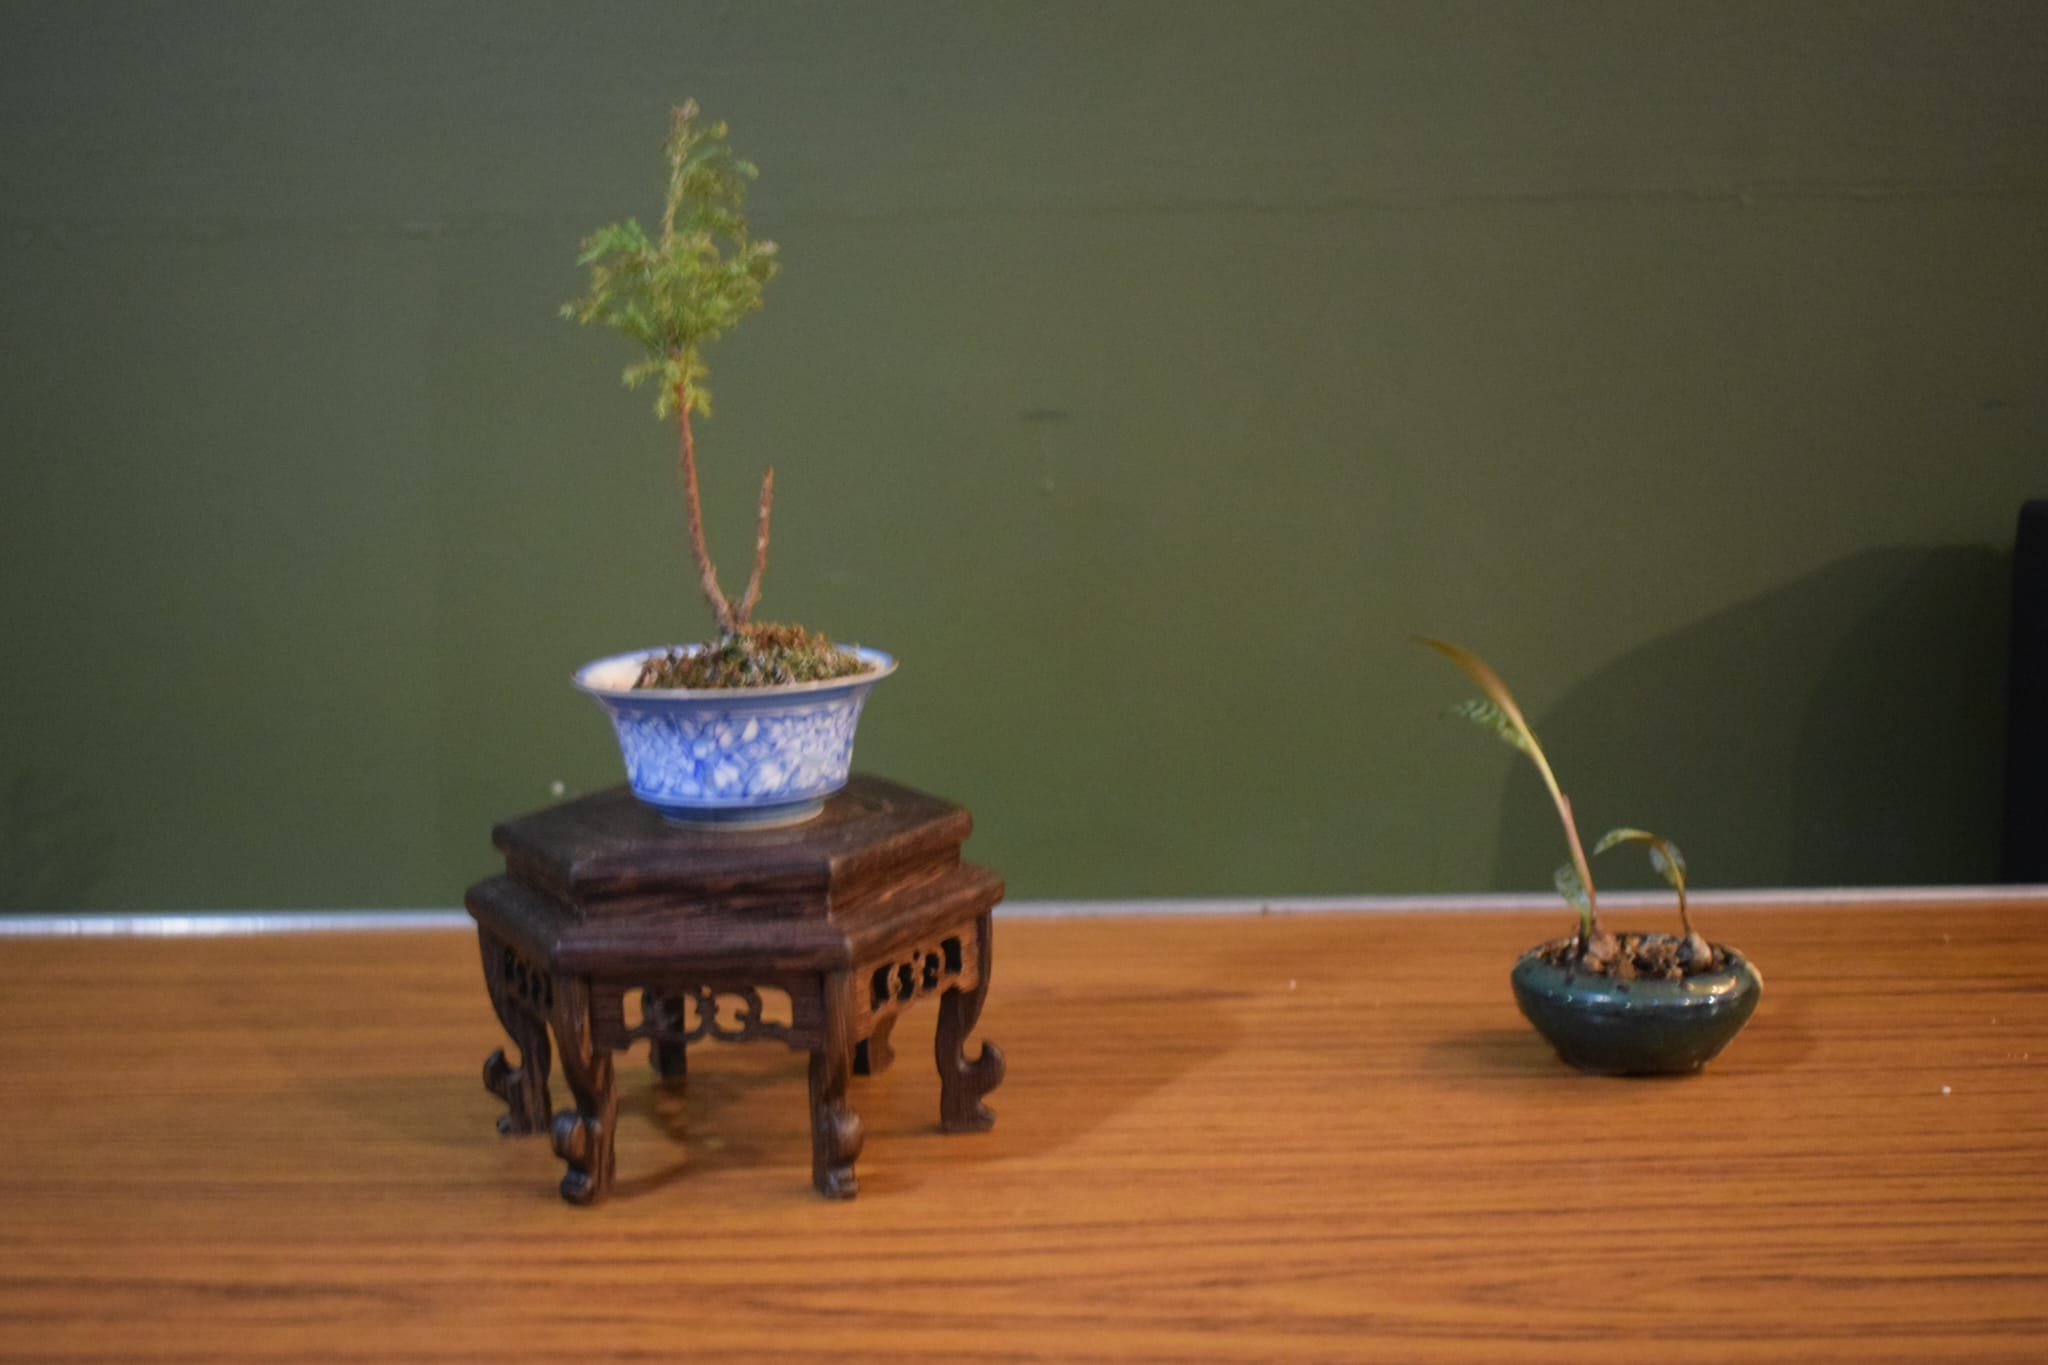
\includegraphics[width=1.0\textwidth]{2025_02/res/contest_novice_edward_cedar}
\centerline{\emph{Edward's Novice Pencil Cedar.}}
\end{minipage}\qquad
\begin{minipage}[b]{.42\textwidth}
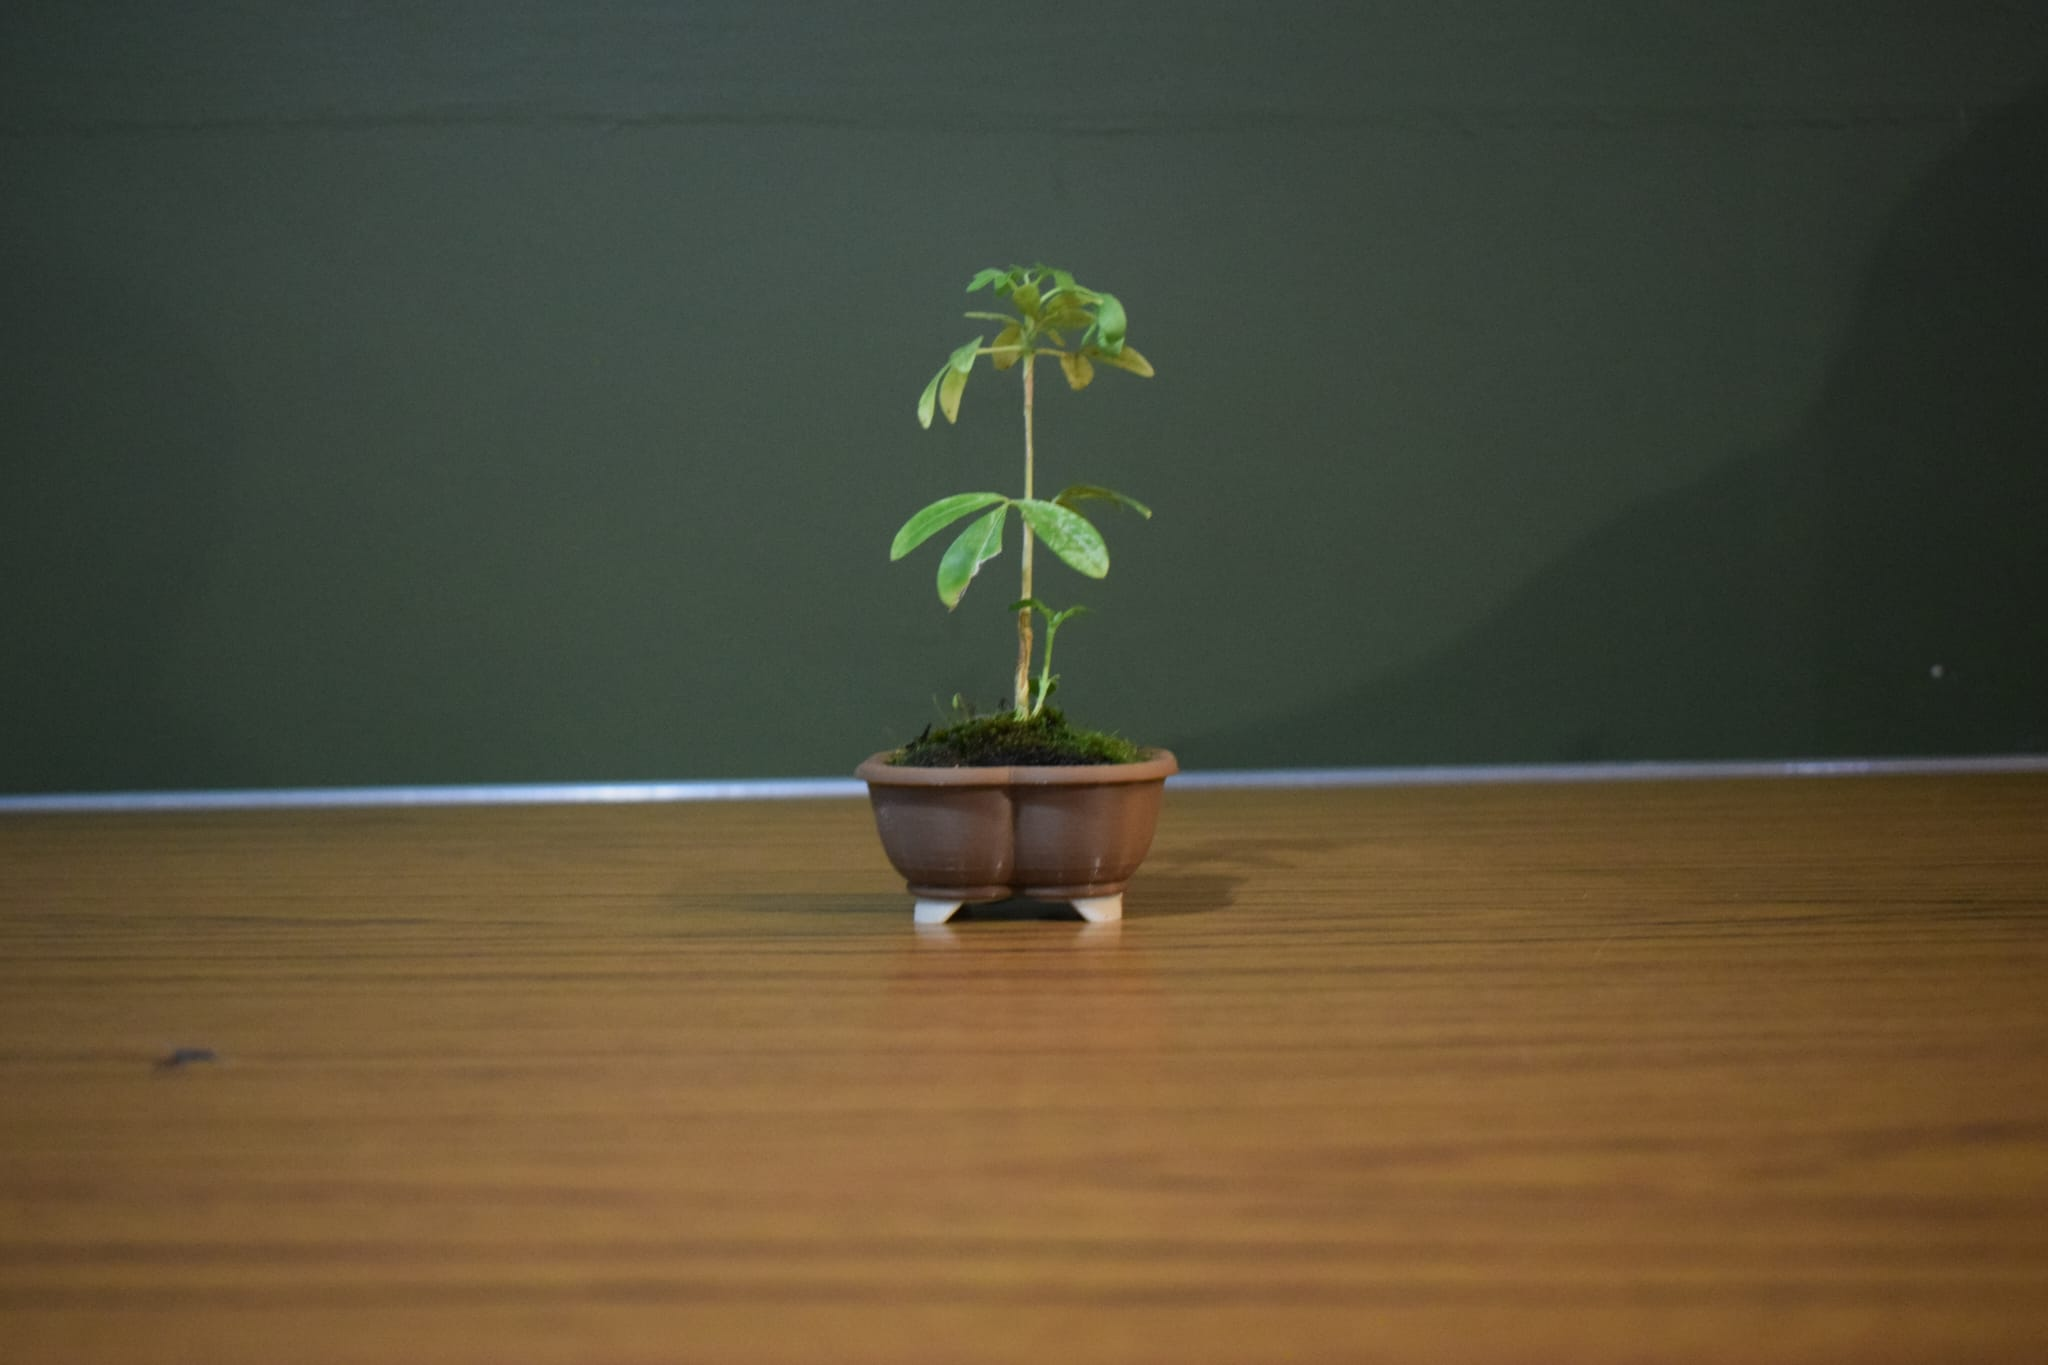
\includegraphics[width=1.0\textwidth]{2025_02/res/contest_novice_stefano_mexican_orange}
\centerline{\emph{Stefano's Novice Mexican Orange.}}
\end{minipage}

\begin{minipage}[b]{.42\textwidth}
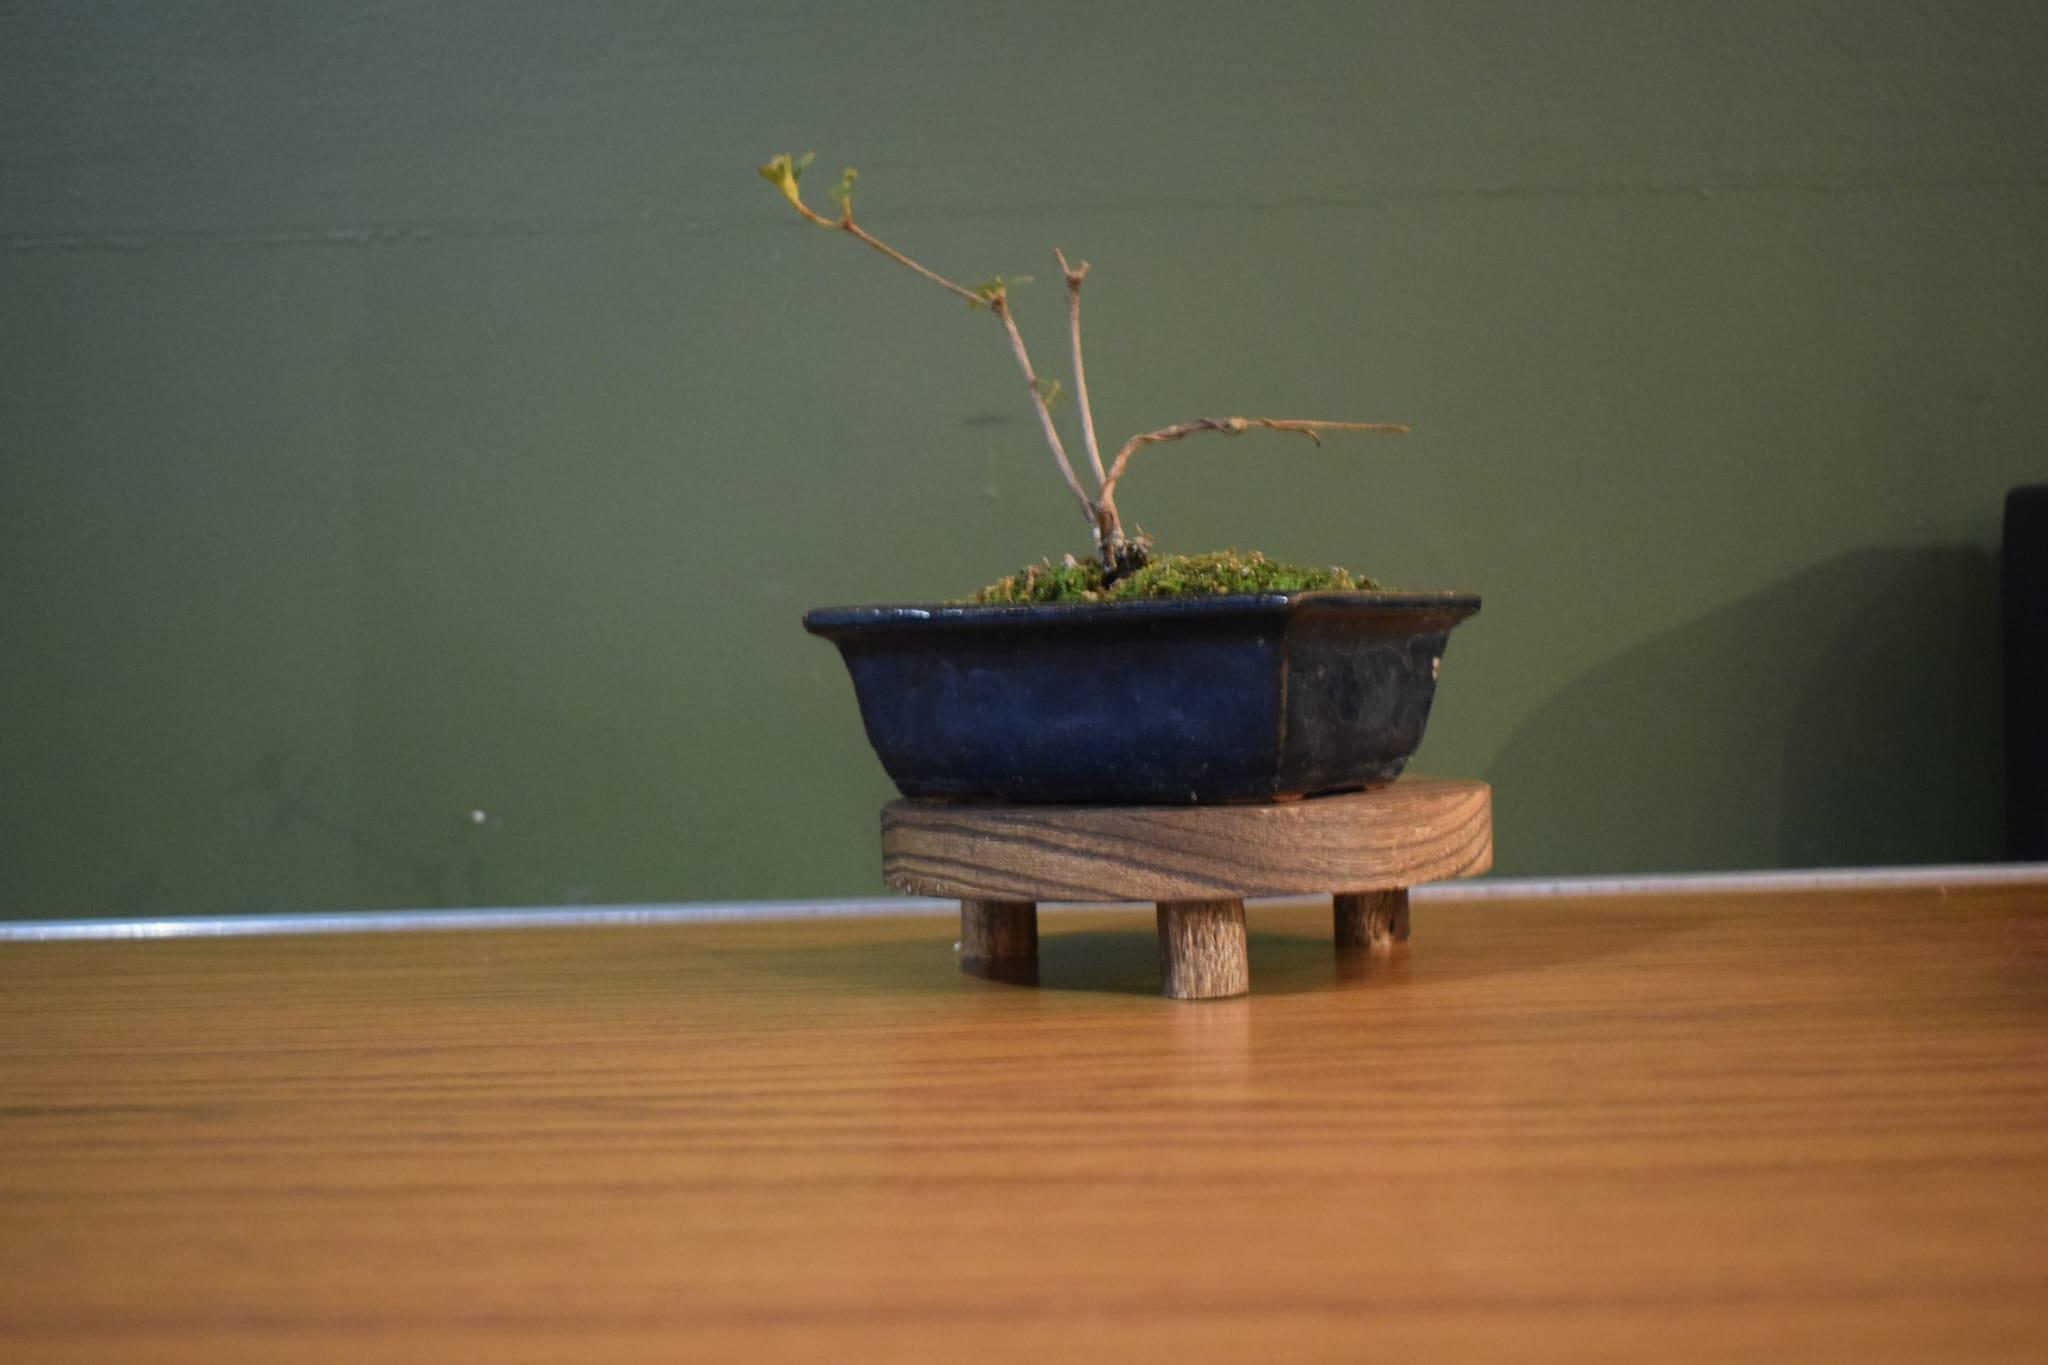
\includegraphics[width=1.0\textwidth]{2025_02/res/contest_novice_laura_azalea}
\centerline{\emph{Laura's Novice Azalea.}}
\end{minipage}\qquad
\begin{minipage}[b]{.42\textwidth}
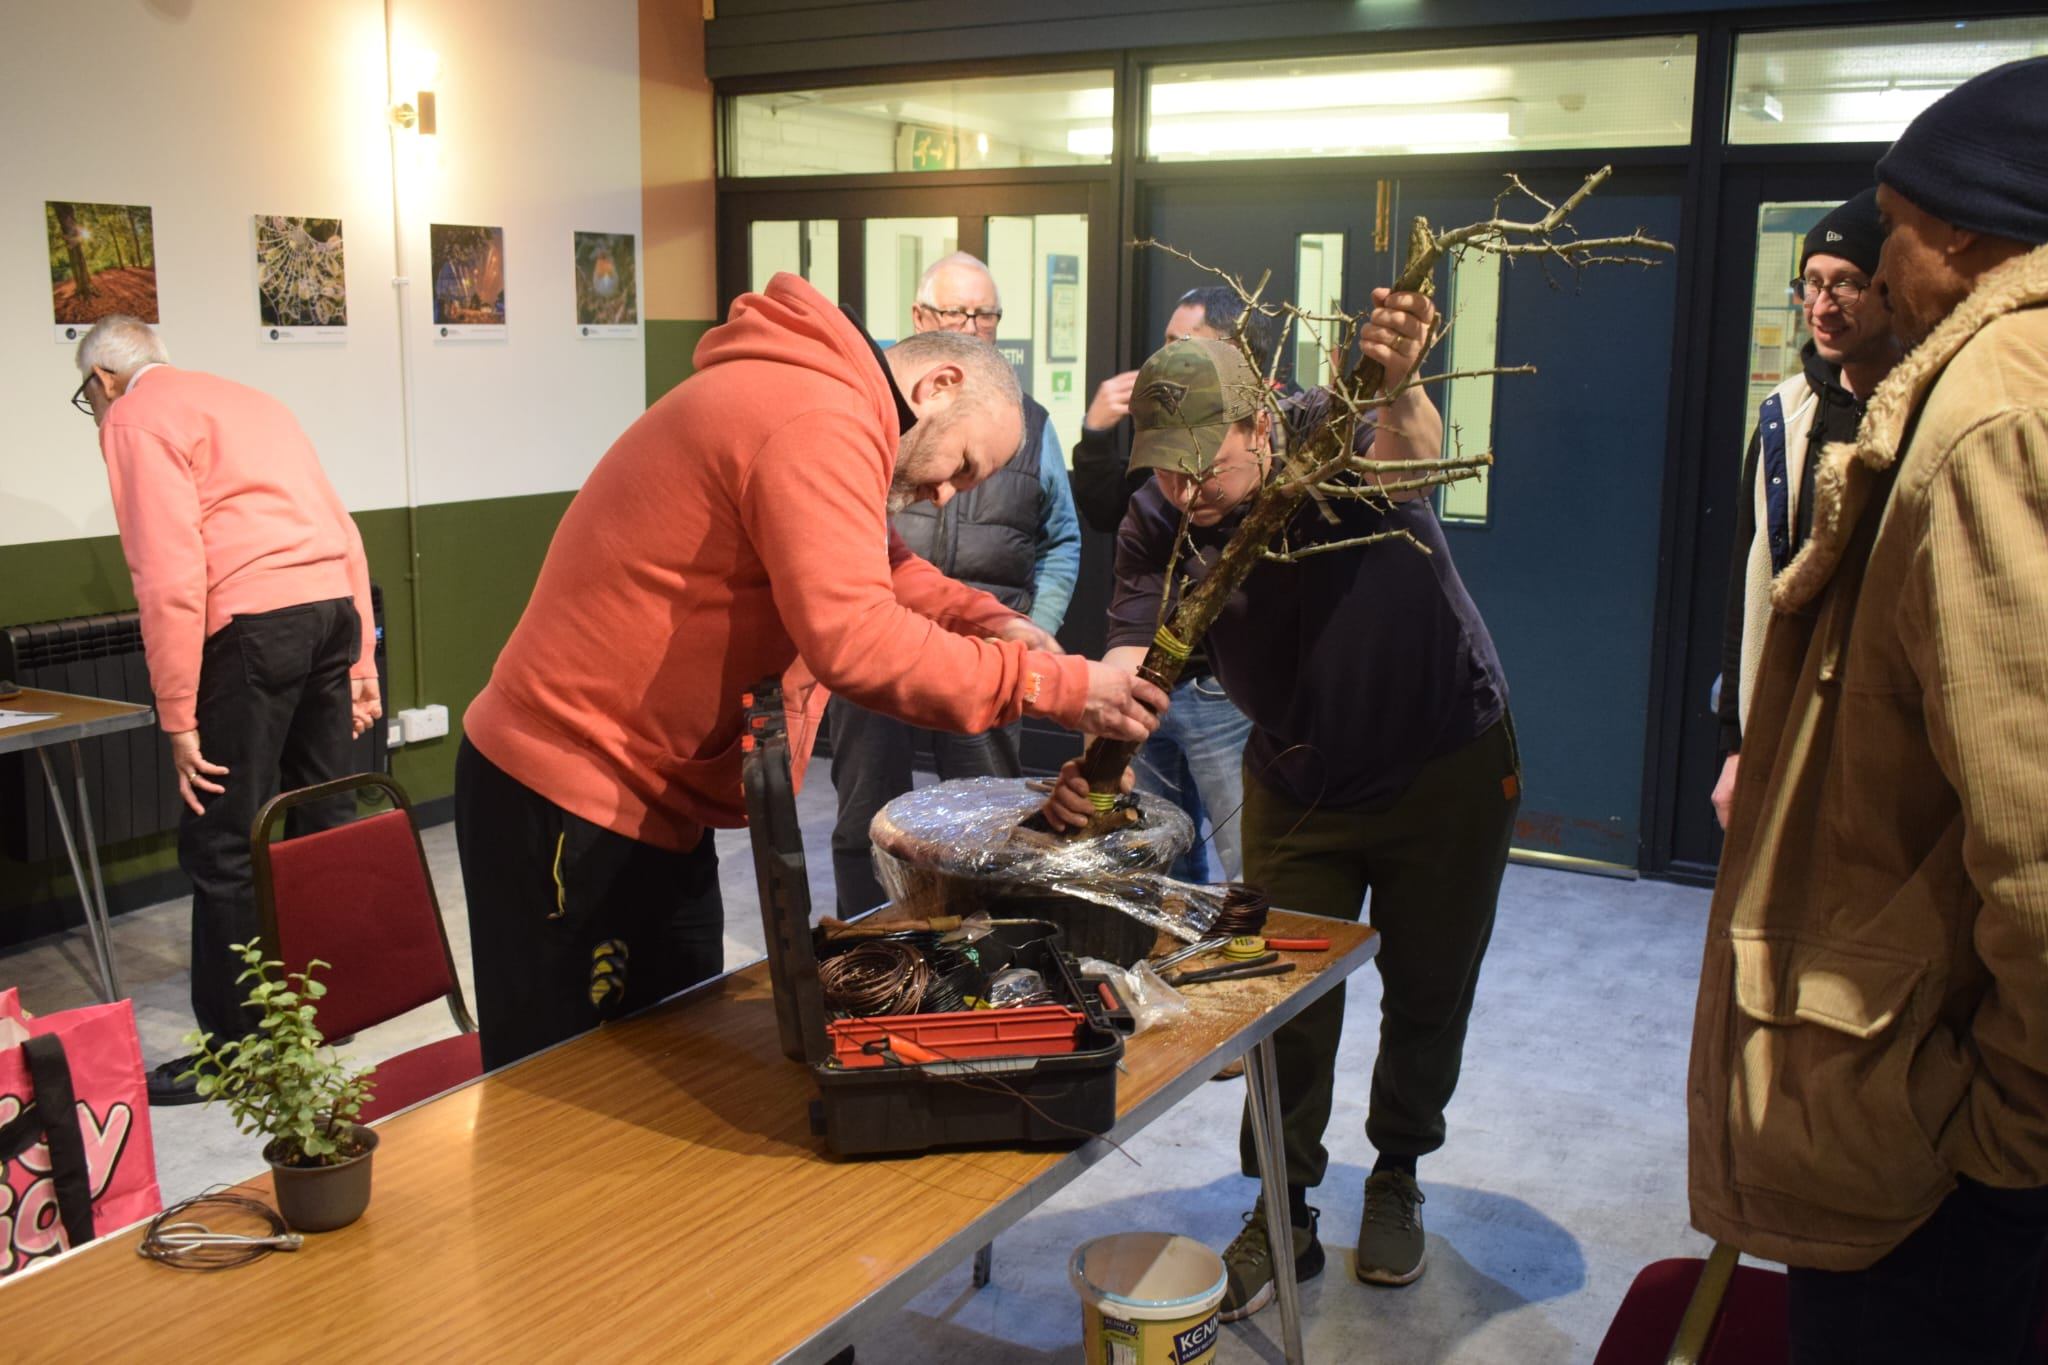
\includegraphics[width=1.0\textwidth]{2025_02/res/gossip_david_bendit}
\centerline{\emph{David bending a hawthorn.}}
\end{minipage}

% \begin{minipage}[b]{.42\textwidth}
% \includegraphics[width=1.0\textwidth]{2025_01/contest_stefano_benjamina.jpg}
% \centerline{\emph{Stefano's Ficus Benjamina.}}
% \end{minipage}
\end{figure*}

\headline{{\textbf{\Large\sffamily The Top Chop:}}\\
          {\textbf{\large\sffamily The Tree of the Month Contest}}}
\label{2025-02-contest}
\noindent
The February meetup of our bonsai club was a delightful celebration of creativity, skill, and the enduring beauty of our miniature trees. 
With the theme \textit{``Carved, Jin's, Uro's'',} members brought forward stunning examples of bonsai artistry, showcasing the intricate techniques of deadwood carving and natural ageing. 
The competition was fierce, but the camaraderie and shared passion for bonsai made the evening truly special.

For those unfamiliar with the rules, here's a quick recap: each attendee can vote on every tree except their own.
Members vote by awarding 1 to 3 marks for four aspects --- trunk/branches, foliage, pot/container, and presentation (aligned with the month's theme) --- with a maximum of 12 points per entry.
This structure ensures a fair and thoughtful evaluation of each tree's unique qualities.

\topic{Tree of the Month}
\noindent 
This month's entries in the \textit{Tree of the Month} category were a testament to the skill and dedication of our members.
Here are the contenders, sorted by scored points:

\begin{enumerate}
    \item \textbf{David Fishwick}'s Cotoneaster (\textit{Cotoneaster microphyllus,} 129 points) --- A masterpiece of carving and presentation, with intricate deadwood features that perfectly embodied the month's theme.
    
    \item \textbf{Brendan Gibbs}' Sabina Juniper (\textit{Juniperus sabina,} 126 points) --- A gracefully twisted trunk with sparse foliage and shari along all the trunk embodying the elegance of literati bonsai.

    \item \textbf{Terry}'s Hornbeam (\textit{Carpinus betulus,} 89 points) ---  A weathered, hollow trunk with dramatic branches creating a striking deadwood bonsai.

    \item \textbf{Rory Campbell}'s Olive (\textit{Olea europaea,} 75 points) --- A rugged, asymmetrical trunk with delicate leaves capturing the beauty of naturalistic bonsai.
\end{enumerate}

\noindent 
\textbf{David Fishwick} is the winner of the \textit{Tree of the Month for February 2025} with his charming Cotoneaster --- congratulations on this well\--deserved victory!

\topic{Novice Tree of the Month}
\noindent 
The \textit{Novice Tree of the Month} category is reserved for members who have been part of the club for less than two years, offering a platform to showcase their progress and celebrate their early achievements in the art of bonsai.
This month's entries were a joy to behold, sorted by scored points:

\begin{enumerate}
    \item \textbf{Edward Mason}'s Pencil Cedar (\textit{Juniperus virginiana,} 54 points) --- A graceful and well-composed little tree with accent, showcasing Edward's keen eye for detail and design.
    
    \item \textbf{Stefano Bragaglia}'s Mexican Orange (\textit{Choisya ternata}, 38 points) --- A charming cutting with vibrant foliage and a promising future as it continues to develop.

    \item \textbf{Laura Shantonas}' Azalea (\textit{Rhododendron sp.,} 35 points) --- A delightful entry, with delicate buds that will soon bloom and a sense of natural beauty that shines through.
\end{enumerate}

\noindent 
\textbf{Edward Mason} is the winner of the \textit{Novice Tree of the Month for February 2025} --- well done on this fantastic achievement!

\begin{center}
    $\cdots$
\end{center}

\noindent
This month's competition was a reminder of the endless possibilities within bonsai. 
Whether you're a seasoned enthusiast or a novice, there's always room to grow, learn, and be inspired. 
Let's continue to challenge ourselves, share knowledge, and celebrate each other's successes.

Looking ahead, next month's theme is \textit{``Yamadori, Urban or Wild'',} celebrating trees collected from nature or urban environments.
We can't wait to see the stories and character these trees bring to our next meetup!

Well done to all participants, and thank you to everyone who voted.
Until next time, happy pruning!
\closearticle
